\section{Measuring AC Voltage with an AC to AC power adapter}
\begin{minipage}{\linewidth}
\begin{table}[H]
    \centering
    \caption{AC-AC Voltage Transformator Data }
    \label{tab:voltage transformator }
    \small
    \begin{tabular*}{\linewidth}{@{\extracolsep{\fill}}ccc}
    \textbf{V (input) (V)} &\textbf{I (mA)} &\textbf{V(output) (mV)} \\\midrule
    10 &0.59 &3.6 \\
    20 &1.15 &8.6 \\
    30 &1.7 &12.8 \\
    40 &2.25 &16.9 \\
    50 &2.8 &21.2 \\
    60 &3.4 &25.3 \\
    70 &3.96 &29.6 \\
    80 &4.52 &33.6 \\
    90 &5 &38 \\
    100 &5.67 &42.2 \\
    110 &6.21 &46.4 \\
    120 &6.77 &51 \\
    130 &7.38 &55.2 \\
    140 &7.9 &59.1 \\
    \bottomrule
    \end{tabular*}
\end{table}
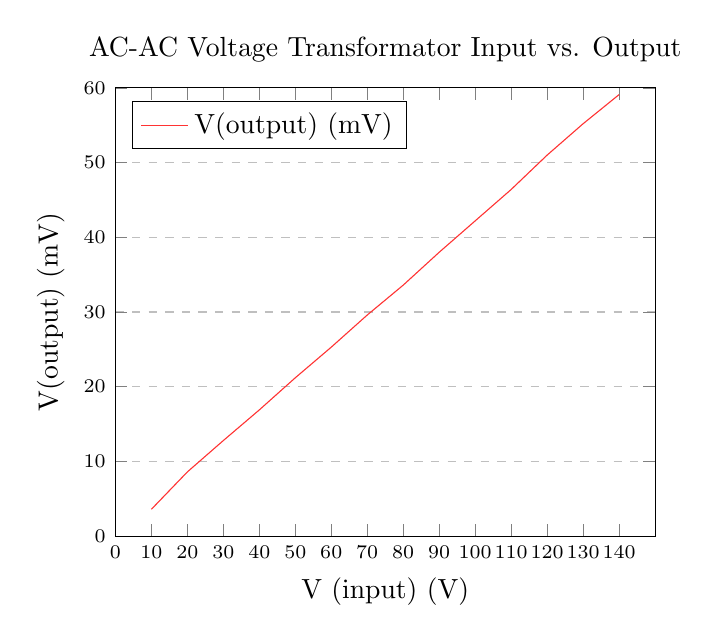
\begin{tikzpicture}
    \begin{axis}[
    title={AC-AC Voltage Transformator Input vs. Output},
    ticklabel style={font=\scriptsize},
    xlabel={V (input) (V)},
    ylabel={V(output) (mV)},
    xmin=0, xmax=150,
    ymin=0, ymax=60,
    xtick={0,10,20,30,40,50,60,70,80,90,100,110,120,130,140},
    ytick={0,10,20,30,40,50,60},
    legend pos=north west,
    ymajorgrids=true,
    grid style=dashed,
    xmajorgrids=false
]
    \addplot[
        color=red!80,
        mark=circle,
    ]
    coordinates {
        (10,3.6)(20,8.6)(30,12.8)(40,16.9)(50,21.2)(60,25.3)(70,29.6)(80,33.6)(90,38)(100,42.2)(110,46.4)(120,51)(130,55.2)(140,59.1)
    };
    \addlegendentry{V(output) (mV)}
    \label{fig:V in-out}
    \end{axis}
\end{tikzpicture}
\end{minipage}

\subsection{AC-AC Power Adapter Schematic}
The circuit is designed to measure AC voltage using an Arduino, an AC-AC power adapter, and a voltage divider. The AC-AC adapter supplies the input voltage (\(V_{\text{in}}\)) to the circuit. The voltage divider, made of resistors \(R_1\) and \(R_2\), steps down the AC voltage to a safe level for the Arduino’s 0-5V input range. The resistors are selected to ensure the voltage stays within the Arduino’s limits.

To allow the Arduino to read both positive and negative portions of the AC waveform, the signal is biased to a 2.5V reference using resistors \(R_3\) and \(R_4\). Capacitor \(C_1\) filters high-frequency noise, ensuring clean signal measurement. A coupling capacitor (\(C_2\)) isolates the DC bias while passing the AC signal to the Arduino’s analog input, where it is digitized for further analysis. This setup enables safe, accurate measurement of AC voltage for energy monitoring.

��\begin{figure}[H]

    \begin{minipage}{\linewidth}

        \begin{center}

            \begin{circuitikz}[scale=0.8, transform shape] % Scale and avoid shape deformation

                % AC-AC Adapter

                \draw (0,4) node[vsource, rotate=-90] (AC) {}

                    (AC.north) node[above=0.3cm] {$\sim$ AC-AC Adapter};



                % First Resistor (R1) in Voltage Divider

                \draw (AC.south)

                      to[R=$R_1$, *-*] (0,2) coordinate (R1R2);



                % Second Resistor (R2) in Voltage Divider

                \draw (R1R2) to[R=$R_2$, *-*] (0,0) coordinate (ground);



                % Capacitor (C1) to Filter Signal

                \draw (R1R2) -- (2,2)

                      to[C=$C_1$] (2,0) -- (ground);



                % Reference Voltage Bias with Resistors (R3 and R4)

                \draw (3,4) to[R=$R_3$] (3,2) coordinate (bias)

                            to[R=$R_4$] (3,0);

                \draw (3,0) node[ground] {};



                % Connect Bias Point to Voltage Divider Output via Coupling Capacitor (C2)

                \draw (R1R2) -- (1,2) to[C=$C_2$] (1.5,2) -- (bias);



                % Arduino Analog Input

                \draw (bias) -- (5,2) node[right, xshift=0.3cm] {Arduino Analog Pin};



                % Labels

                \node at (1,3.5) {$V_{in}$}; % Adjusted label position

                \node at (4.5,2.5) {$V_{out}$ (0-5V range)}; % Adjusted label position

                \node at (1.6,0.5) {Ground}; % Adjusted label position



            \end{circuitikz}

        \end{center}

        \caption{Voltage Divider with Filtering and Biasing for Arduino Analog Input}

        \label{fig:voltage-divider}

    \end{minipage}

    \end{figure}


